\par{The perimeter kernel, despite what its name suggests, does not necessarily operate on elements 
    at the perimeter of the matrix. Figure \ref{PerimeterKernel2} demonstrates the areas of the matrix where the 
    perimeter kernel computes.}

\begin{figure}[!h]
    \centering
    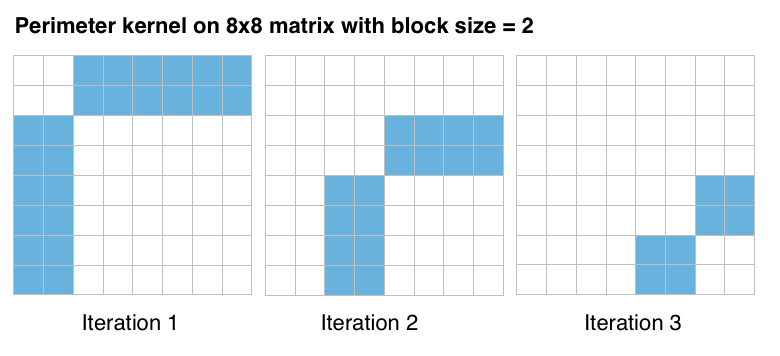
\includegraphics[width=0.6\textwidth]{figures/PerimeterKernel2.png}
    \caption{Perimeter kernel algorithm on 8x8 matrix with block size = 2.}
    \label{PerimeterKernel2}
\end{figure}

\par{This kernel, like the other two kernels, is enqueued multiple times by the host, each 
    time to operate on a different portion of the matrix, as shown above.}

\par{At each iteration of the loop in the host code, the total number of work-groups is decreased by one. 
    Eventually, in the last iteration of the loop, only 1 work-group will be enqueued. 
    Since work-groups are scheduled in parallel on the Xeon Phi and Xeon CPU, 
    this means that the parallelism of the algorithm reduces as the computation proceeds.}

\par{The opposite is true for the GPU. The number of work-items per work-group increases for greater block sizes. 
    This increases the parallelism of the algorithm on the GPU. In both cases, however, 
    there is guaranteed to be at least some under-utilisation of the hardware threads. 
    Table \ref{tab:lu2} summarises some of the relevant parameters.}

\begin{table}[!h]
    \centering
    \begin{tabular}{| l | l | l | l |}
    \hline
    \emph{Block Size} & \emph{Data Size / Work Group} & \emph{Starting Number of Work Groups} & \emph{\#Work-Items / Work-Group} \\ \hline
    2 & 2x2 & 2047 & 4 \\ \hline
    4 & 4x4 & 1023 & 8 \\ \hline
    8 & 8x8 & 511 & 16 \\ \hline
    16 & 16x16 & 255 & 32 \\ \hline
    32 & 32x32 & 127 & 64 \\ \hline
    64 & 64x64 & 63 & 128 \\ \hline
    \end{tabular}
    \caption{Perimeter Kernel Summary.}
    \label{tab:lu2}
\end{table}

\par{The performance of this kernel can be explained as a compromise between a number of parameter changes. 
    Firstly, a greater block size will decrease the number of work-groups and increase the number of work-items per work-group. 
    For example, with a block size of 32, there will be a maximum of 127 work groups, 
    reducing to 1 work-group as the computation proceeds, but there will be 64 work-items per work-group. 
    In this case, the algorithm would be under-utilising the hardware threads of the Xeon CPU and the Xeon Phi, 
    but exploiting the parallelism available in the GPU.}

\par{A greater block size reduces the overhead of loading data from global to local memory, 
    since more data is loaded to memory at each execution. For each greater block size, 
    the total number of floating-point operations approximately doubles.}

\begin{figure}[!h]
    \centering
    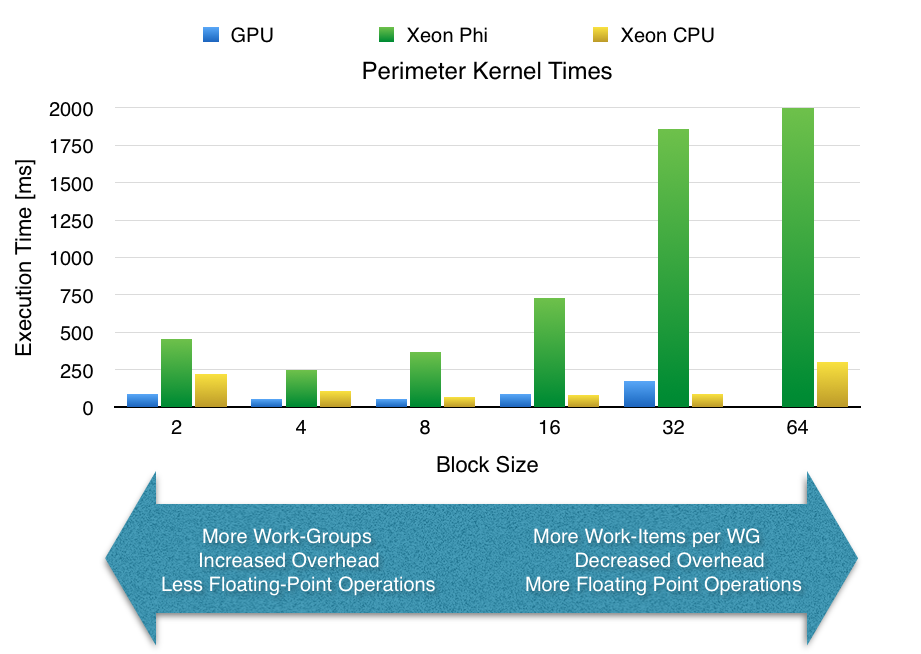
\includegraphics[width=0.6\textwidth]{figures/PerimeterKernel1.png}
    \caption{4096x4096 Perimeter Kernel Times.}
    \label{PerimeterKernel1}
\end{figure}

\par{Figure \ref{PerimeterKernel1} summarises these points. An increase in block size effectively 
    reduces the parallelism of the algorithm on the Xeon CPU and Xeon Phi, but reduces 
    the overhead incurred from high-latency data transfers. For the GPU, the increase 
    in block size gives rise to a higher level of parallelism, since work-items are scheduled 
    in parallel on the cores within each streaming multiprocessor. Unfortunately, the fact that the 
    total number of floating point operations increases according to the block size skews the results.}

